\chapter{Validación de la Solución}

% Demostración de cómo la solución resuelve el problema
% Dependiendo de la naturaleza del problema / solución:
% - Uso de la aplicación desarrollada en un contexto real reportando los resultados
% - Simulación de uso con un caso representativo
% - Encuesta a usuarios finales
% Dependiendo de la longitud, la validación puede ser una sección al final del capítulo de solución o un capítulo independiente

\section{Antecedentes de datos de prueba}

\todo[inline]{Explicar datos de sloan}

Una vez lista la implementación de la mayor parte del sistema y los algoritmos de ARL, se procedió a realizar una prueba de concepto con datos reales. El objetivo final del sistema de ARL es poder ser aplicado a datos de líneas espectrales de diversos orígenes y características; sobre todo en observaciones sobre bandas de baja frecuencia, donde una mayor densidad de presencia de líneas hace más difícil el trabajar directamente sobre ellas, como suele ser el caso en bandas de frecuencia más alta.

Sin embargo, se decidió realizar la prueba de concepto de este proyecto sobre datos del \textit{Sloan Digital Sky Survey (SDSS)} por las siguientes razones:

\begin{enumerate}
\item Si bien el universo de líneas presentes en cada espectro es bastante reducido (48 líneas), la mayoría de estas se encuentran bien identificadas.
\item Las líneas presentes en el espectro óptico son bien conocidas, y en general se posee información completa sobre sus características, tales como su temperatura.
\end{enumerate}

Ahora bien, hubo que tener en mente de forma constante que se está trabajando con un universo reducido de ítemes (líneas espectrales) al momento de analizar los resultados de estas pruebas.

Para acceder a los datos de \textit{SDSS} se utilizó la interfaz web del sistema \textit{CasJobs}, que recibe consultas en lenguaje SQL y guarda los resultados en una base de datos asociada a la cuenta del usuario. En particular se hizo uso de los datos del \textit{data release 7 (DR7)}, que es el último en contener tablas con información específica sobre las líneas espectrales.

En particular, se utilizó dos tablas pertenecientes al DR7: \textit{SpecObj} y \textit{SpecLineAll}. 

La tabla \textit{SpecObj} contiene información de los objetos astronómicos sobre los cuales se ha realizado mediciones espectroscópicas. De esta tabla se extrayeron los siguientes campos:

\begin{itemize}
\item \textbf{specObjID}: Identificador del objeto astronómico.
\item \textbf{zStatus}: Flag que indica el método mediante el cual se calculó el \textit{redshift} del objeto.
\item \textbf{objTypeName}: El tipo de objeto (e.g. galaxia, estrella, quasar), determinado mediante imágenes.
\item \textbf{specClass}: El tipo de objeto, determinado mediante su espectro.
\item \textbf{mag\_0}. \textbf{mag\_1} y \textbf{mag\_2}: Magnitud de emisión en tres frecuencias distintas.
\item \textbf{z}: \textit{Redshift} del objeto.
\item \textbf{zErr}: Error de \textit{Redshift} del objeto.
\end{itemize}

A su vez, la tabla \textit{SpecLineAll} contiene información sobre cada una de las líneas presentes en cada uno de estos objetos. De esta tabla se extrayeron los campos:

\begin{itemize}
\item \textbf{SpecLineID}: Código identificador único de línea espectral.
\item \textbf{wave}: Posición central de la línea espectral observada, en longitud de onda (Armstrongs), dentro del espectro.
\item \textbf{waveErr}: Error en la posición central de la línea espectral.
\item \textbf{restWave}: Posición central de la línea espectral teórica o medida en laboratorio.
\item \textbf{lineID}: Identificador de línea espectral (identifica una línea de una especie en particular).
\item \textbf{category}: 1 si la línea se detectó mediante el uso de ajuste de modelos luego de aplicar un filtro (o \textit{transformada wavelet}) con el fin de determinar el \textit{redshift} de las líneas de emisión y 2 si la línea se detectó una vez que el objeto fue clasificado y su \textit{redshift} determinado.
\item \textbf{height}: Altura de la función gaussiana ajustada a la línea.
\item \textbf{heightErr}: Error de la función gaussiana ajustada a la línea.
\item \textbf{ew}: Ancho equivalente de la línea (una medida de su intensidad).
\item \textbf{ewErr}: Error del ancho equivalente.
\item \textbf{z}: \textit{Redshift} de la línea.
\item \textbf{zErr}: Error de \textit{redshift}.
\end{itemize}

Ahora bien, la tabla \textit{SpecObj} del DR7 de SDSS posee en total de 1053144 filas. Esto indica que aquel \textit{data release} contiene información espectroscópica de más de un millón de objetos. Cabe recalcar que el caso general del sistema de ARL aplicado a lineas espectrales asume que cada transacción corresponde a una observación o lectura de un espectro de frecuencias; y, por tanto, varios espectros pueden estar asociados a un mismo objeto astronómico. Sin embargo, dado que para el caso de los datos de SDSS puede que las líneas pertenecientes a cada objeto se hayan obtenido en diversas observaciones, se tomará cada \textbf{objeto} como una transacción, y no la observación particular de un objeto.

Por lo tanto al hacer una operación \textit{JOIN} entre las tablas \textit{SpecObj} y \textit{SpecLineAll}, se obtendrá la lista de todas las líneas espectrales con información del objeto astronómico del cual provienen. La idea es, entonces, utilizar cada uno de los objetos como una transacción, y las líneas asociadas a cada uno de ellos como sus ítems. Se utilizará el campo \textit{lineID} de la tabla \textit{SpecLineAll} como identificador de cada uno de estos ítemes; dado que dos líneas asociados a distintos objetos pueden tener el mismo valor en \textit{lineID}, cosa que no ocurre con el identificador único \textbf{SpecLineID}. 

En efecto, existe en el DR7 una tabla llamada \textit{SpecLineNames} que enumera los 49 valores que puede tomar el campo \textit{lineID}. Cada uno de estos corresponde a una línea de una especie en particular. Algunos de estos valores son:

\begin{tabular}{l l}
\textbf{Valor} & \textbf{Nombre} \\
1857 & AlIII\_1857 \\
8500 & CaII\_8500 \\
8544 & CaII\_8544 \\
8665 & CaII\_8665 \\
1335 & CII\_1335 \\
2326 & CII\_2326 \\
\end{tabular}

A continuación se numeran los objetos de la tabla \textit{SpecObj} según el tipo de objeto determinado mediante su espectro (campo \textit{specClass}).

\begin{tabular}{c l c}
\textbf{\textit{specClass}} & \textbf{Tipo de objeto} & \textbf{Número de objetos}\\
0 & Desconocido & 11566 \\
1 & Estrella & 85564 \\
2 & Galaxia & 807118 \\
3 & Cuasi-estelar (\textit{quasar}) & 94994 \\
4 & \textit{Quasar} de alto \textit{redshift} & 7584 \\
6 & Estrella tardía & 46318 \\
\end{tabular}

\section{Selección y pre-procesamiento de datos}

\todo[inline]{Filtrado, de objetos, de líneas. Gráficos.}

Para fines de esta prueba de concepto y validacíón del sistema se escogió realizar la extracción de reglas de asociación a partir de objetos de tipo estelar (\textit{specClass} 1 o 6), principalmente debido a que para objetos de este tipo el \textit{redshift} del objeto en general debería ser más coherente que el \textit{redshift} detectado por línea o espectro que en el caso de, por ejemplo, objetos de tipo galáctico.

En total, existen 52570585 líneas asociadas a los 131882 objetos de tipo estelar presentes en el \textit{data release 7}. Esto supone un claro problema técnico, dado que el sistema \textit{CasJobs} no permite descargar tablas de tal envergadura. Por lo tanto, debe realizarse un proceso de selección lo más sistemático posible. 

En primer lugar, se consideró el conjunto de 131882 objetos de tipo estelar. En la Figura \ref{fig:stelar_obj_redshift} se puede apreciar una selección del histograma del \textit{redshift} de estos objetos. Se puede apreciar que la mayoría de los objetos se encuentran cercanos a 0 y unos pocos se encuentran distribuidos en valores mayores. Se decidió por tanto, eliminar estos objetos de mayor \textit{redshift} (y por tanto más lejanos) con el fin de trabajar sólo con aquellos objetos más cercanos. Se decidió por utilizar solo los objetos que tengan un \textit{redshift} menor que 0.002.

\begin{figure}[h!]
\begin{center}
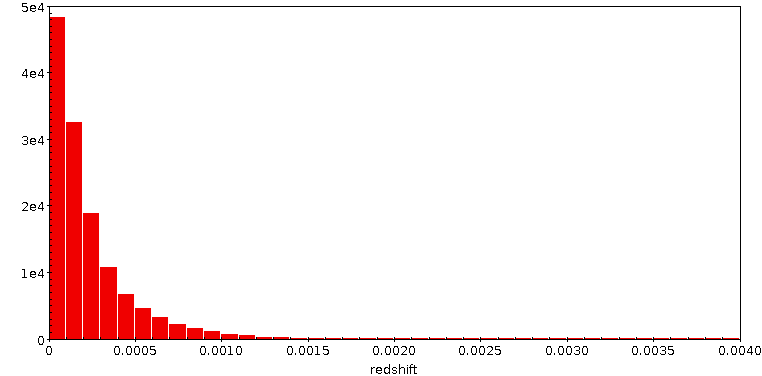
\includegraphics[width=0.9\textwidth]{imagenes/stelar_obj_redshift_hist.png}
\end{center}
\vspace*{-5mm}
\caption{Histograma de \textit{redshift} de objetos estelares.}
\label{fig:stelar_obj_redshift}
\end{figure}

Ahora bien, con el fin de reducir de forma más considerable el número de líneas a analizar, se decidió filtrar estas y dejar sólo las más brillantes. Para esto, se utilizó los valores de \textit{ancho equivalente (ew)} de cada una de las líneas, y se calculó una nueva medida a la que se denominó \textit{razón señal a ruido (SNR)} que consiste en la razón entre el ancho equivalente y su error (\textit{ewErr}). Para comprobar si este valor es un filtro efectivo del número de líneas, se tomo una muestra de 1 millón de líneas del total asociado a objetos estelares, y se produjo el histograma acumulativo de la Figura \label{fig:stelar_obj_snr}. Observando esta figura, se puede apreciar que, en efecto, esta nueva medida introducida es un parámetro efectivo de selección de líneas (cerca del 20\% de las líneas de la muestra tiene un SNR mayor que 5).

\begin{figure}[h!]
\begin{center}
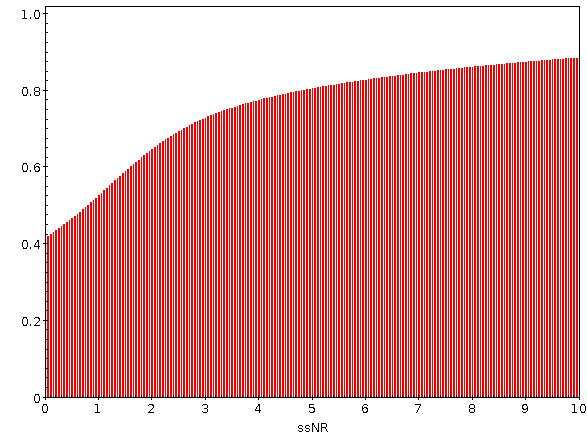
\includegraphics[width=0.9\textwidth]{imagenes/stelar_obj_snr_hist.png}
\end{center}
\vspace*{-5mm}
\caption{Histograma acumulativo de líneas asociadas a objetos estelares por su \textit{SNR}.}
\label{fig:stelar_obj_snr}
\end{figure}

Seleccionando, del total de líneas asociadas a objetos estelares, aquellas que estén asociadas a objetos con redshift menor que 0.002 y que tengan un \textit{SNR} mayor que 5, se obtiene un total de 1189817 líneas asociadas a 120250 objetos estelares. 

Sin embargo, algunas de estas líneas no poseen un identificador \textit{lineID} y otras que sí lo poseen se encuentran mal identificadas. La razón de por qué ocurre esto se muestra en la Figura \label{fig:speclinez_hist}. Como ahí se puede apreciar, existe un gran número de líneas cuyo \textit{redshift} (indicado por el campo \textbf{z} de la tabla \textit{SpecLineAll}) tiene como valor ${-9999}$. Esto no tiene sentido alguno desde el punto de vista físico, e indica sencillamente un valor nulo o inexistente.

\begin{figure}[h!]
\begin{center}
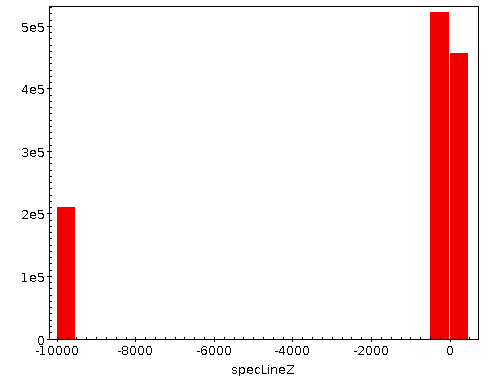
\includegraphics[width=0.9\textwidth]{imagenes/speclinez_hist.png}
\end{center}
\vspace*{-5mm}
\caption{Histograma de \textit{redshift} de las líneas espectrales seleccionadas.}
\label{fig:speclinez_hist}
\end{figure}

Incluso en muchas las 979173 líneas que resultan de filtrar aquellas que poseen valores nulos de \textit{redshift}, este valor aún así no concuerda con el \textit{redshift} del objeto; tomando el \textit{redshift} de la línea valores que llegan hasta 5, cuando el del objeto correspondiente se encuentra mucho más cercano a 0, como se observa en la Figura \label{fig:specobjz_vs_speclinez}

\begin{figure}[h!]
\begin{center}
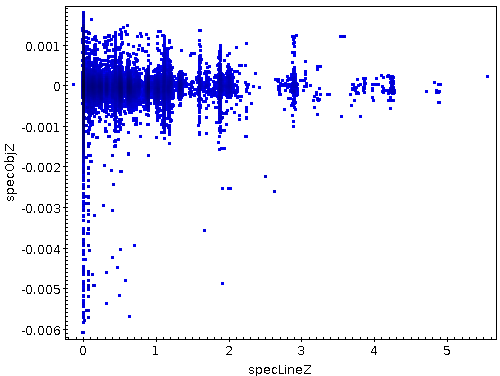
\includegraphics[width=0.9\textwidth]{imagenes/specobjz_vs_speclinez.png}
\end{center}
\vspace*{-5mm}
\caption{Gráfico de \textit{redshift} de las líneas espectrales seleccionadas vs el del objeto al que pertenecen.}
\label{fig:specobjz_vs_speclinez}
\end{figure}

Dado que el identificador de línea \textit{lineID} corresponde a una aproximación del la posición central de la línea espectral teórica o medida en laboratorio en Armstrongs (campo \textit{restWave} de la tabla \textit{specLineAll}) al entero más cercano, y que este último valor se calcula a partir de la posición central observada (campo \textit{wave}) y el \textit{redshift} de la línea (campo \textit{z}), se entiende que si el valor de \textit{redshift} no es el correcto, entonces finalmente el identificador de línea tampoco lo será.

Por eso, como parte del pre-procesamiento de los datos se prefirió, para aquellas líneas con \textit{lineID} inexistente o \textit{redshift} erróneo, volver a calcular un \textit{restWave} utilizando el \textit{redshift} del objeto en vez del de la línea; y de ahí incluir el \textit{lineID} resultante de aproximar el 

\section{Resultados}

\todo[inline]{Mostrar las reglas de asociación resultantes con tablas, gráficos, grafos, figuritas, pegatinas, etc...}